% this file is called up by thesis.tex
% content in this file will be fed into the main document

%: ----------------------- name of chapter  -------------------------
\chapter{An End-to-end Recurrent Neural Network Approach with Even Chance Training}\label{cp:endtoend} % top level followed by section, subsection


As recapped in Section~\ref{sec:2-rnnpm} that by now there are basically four approaches for ACE:
\begin{itemize}
\item local feature extraction - global smoothing \cite{fujishima1999realtime,sheh2003chord}
\item local classification - global smoothing \cite{humphrey2012rethinking};
\item local feature learning - global classification - global smoothing \cite{boulanger2013audio,sigtia2015audio};
\item local feature learning - local classification - global smoothing \cite{zhou2015chord}.
\end{itemize}
All of these approaches incorporate a ``global smoothing'' stage after classification. This is a step that requires prior domain knowledge which does not belong to the deep learning approach. Moreover, all these approaches, including those tradition ones, do not explicitly take into account the fact that the chords are distributed in a highly uneven way and that the chord classification problem is actually a skewed classes problem. If the similar approaches are used for LVACE, it is very probable that the systems will over-fit the chord types that are highly over-represented.

This chapter is going to study an ``end-to-end'' approach that tries to employ a new neural network training scheme to achieve a more balanced performance on both common and uncommon chords, and on the other hand avoid the need of ``global smoothing'' altogether. The system presented here belongs to the ``local feature extraction - global classification'' category.


%: ----------------------- contents from here ------------------------
\section{System Overview}\label{sec:4-sysover}
Figure \ref{fig:4-sysover} shows the system overview, which mainly contains a feature extraction module and a BLSTM-RNN sequence decoding module. The former is the same as the feature extraction process presented in Chapter~\ref{cp:ghmm}.

\begin{figure}[htb]
\centering
\includegraphics[width=0.4\columnwidth]{4/figures/sys.pdf}
\caption{BLSTM-RNN end-to-end ACE System Overview. The raw audio is feature extracted into a piece of chromagram or notegram, and then decoded by a BLSTM-RNN into a segmented chord sequence.}
\label{fig:4-sysover}
\end{figure}

\section{Implementation}\label{sec:4-blstm}
The key module in this system is the BLSTM-RNN. This section will first briefly discuss RNN's variable-length sequence training, and then elaborate on the implementation of the BLSTM-RNN.

\subsection{RNN Training}
A RNN can model the conditional probability of a label sequence $l$ given its corresponding input feature sequence $x$. Let's define the label alphabet as $L$, and let both $x$ and $l$ have the same length $T$ in the unit of time. The conditional probability $p(l|x)$ modeled by the RNN can be written as:

\begin{equation}\label{eq:4-rnnprob}
	p(l|x) = \prod_{t=1}^T y_{l_t}^t  \quad\quad l\in L \quad and \quad |l| = |x|
\end{equation}

where $l_t$ is the $t^{th}$ element of $l$ and $y_{l_t}^t$ is the probability of predicting label $l_t$ at time $t$ given $x$. At time $t$, $y_{l_t}^t$ can also be written as $p(l_t|x)$, which is the value of the $l^{th}$ slot of RNN prediction at time $t$. This RNN can be trained using a maximum likelihood approach by updating the network weights towards a direction that increases the conditional probability of ground truth sequences given their input representation sequences. Thus the cost function will be the same as equation \ref{eq:4-rnnprob} (or the logarithm of it) given both $l$ and $x$ are in the training set.

\subsection{BLSTM-RNN Architecture} \label{sec:blstmrnnarch}
Figure \ref{fig:4-blstm} shows the graphical model of the BLSTM-RNN, which has a forward and a backward hidden layer both with 800 LSTM units. The input layer has the same dimension of the input feature. The output layer is a \textit{\#-chord-way} softmax layer. (The softmax layer is suitable for multi-class classification problem because its outputs are posterior probabilities of all chords in the vocabulary conditioned on the input bass-treble chromagram.)

\begin{figure}[htb]
	\centering
	\includegraphics[width=0.6\columnwidth]{4/figures/blstm.pdf}
	\caption{The BLSTM-RNN. Both the forward and backward hidden layers contain 800 LSTM units}
	\label{fig:4-blstm}
\end{figure}

\subsection{Vocabulary and Datasets}
The large vocabulary supported by the proposed system are again the \textit{SeventhsBass} described in the previous chapters. Also the raw datasets used in the experiments are the same as the Chapter~\ref{cp:ghmm}'s, but the data generation and augmentation schemes are different, which will be described as follows.

\subsection{Data Augmentation}
To generate training data, firstly all raw audios are transformed to bass-treble chromagram and notegram representations. The original segment-wise ground truth annotations are upsampled to become frame-wise annotations with 1-to-1 mappings to their input representations. Due to the absence of phase information in chromagram and notegram, all data can be circularly transposed to 12 keys to yield 12 times the original amount of data \cite{humphrey2012rethinking}.

\subsection{Training and Cross-validation}
Two different training schemes are used. The only difference between them are the way of choosing training cases at each iteration:
\begin{itemize}
	\item completely random (CR): a random training case is chosen.
	\item even chance (EC): a training case of a certain chord type is chosen, and each chord type has an even chance to be chosen.
\end{itemize}
The EC training scheme is inspired by the skewed class sensitive training methods \cite{chawla2004editorial}.
Considering a skewed distribution of chord classes in the training datasets \cite{burgoyne2011expert}, a random sampling scheme like CR will inevitably draw samples based on that same distribution, which causes lack of exposure of uncommon chords. The EC scheme, however, gives each class an equal chance of exposure during the training process. Concretely, the EC scheme is formalized as follows in Algorithm~\ref{alg:4-ectrain}:
\begin{algorithm}[h]
	\caption{EvenChanceTraining}
	\label{alg:4-ectrain}
	\begin{algorithmic}
		\REQUIRE
		training dataset - $(X,y)$;
		number of chord classes - $nclass$;
		early stopping flag - $es$.
		\STATE % empty line
		\STATE $bd$ = BalancedDict($y$, $nclass$)
		\STATE $iter$ = $0$
		\WHILE {$es$ is \FALSE}
		\IF {mod($iter$, $nclass$) is $0$}
		\STATE $coidx$ = random\_shuffle($0$:$nclass$-$1$)
		\ENDIF
		\STATE $tclist$ = $bd(coidx_{mod(iter, nclass)})$
		\STATE draw a random item $e$ from $tclist$
		\STATE update network with $(X,y)_e$
		\STATE $iter$++
		\ENDWHILE
	\end{algorithmic}
\end{algorithm}

The core of this procedure is the ``\textit{BalancedDict}'' which computes for a dictionary of \textit{(track index, chord change position)} tuples indexed by chord classes. It is formalized in Algorithm~\ref{alg:4-bod}:
\begin{algorithm}[h]
	\caption{BalancedDict}
	\label{alg:4-bod}
	\begin{algorithmic}
		\REQUIRE
		labels of training dataset - $y$;
		number of chord classes - $nclass$.
		\STATE % empty line
		\FOR {each class $i$ from $0$ to $nclass-1$}
		\STATE initialize an empty list $bd[i]$
		\ENDFOR
		\FOR {each track index $j$ in $y$}
		\FOR {each frame poistion $k$ in $y[j]$} 
		\IF {$k$ is a chord change position}
		\STATE append ($j$,$k$) to $bd[y[j][k]]$
		\ENDIF
		\ENDFOR
		\ENDFOR
		\RETURN
		$bd$
	\end{algorithmic}
\end{algorithm}

Each entry of $bd$ contains a list of \textit{(track index, chord change position)}. This scheme guarantees an even chance of training for each class, given that each class has at least one case in the training set.

The following describes the remaining training procedures that apply throughout the experiments in both CR and EC schemes:
\begin{itemize}
	\item Each training case contains 500 frames of audio content with ground truth labels (subject to the end-of-track boundary condition);
	\item The network update signal is computed by an Adadelta optimizer \cite{zeiler2012adadelta};
	\item The training is regularized with dropout \cite{srivastava2014dropout} and early-stopping \cite{prechelt1998early};
	\item All dropout probabilities are set to 0.5;
	\item All early-stopping criteria are monitored using the validation error of CNPop20 dataset, which is not in any cross-validation set; The validation cycle is 100 iterations;
	\item The model with the lowest validation loss will be saved, and if the current validation loss is smaller than 0.996 of the best one, the early-stopping patience will increase by 0.3 times the current number of iterations;
	\item Training stops when the patience is less than the current number of iterations.
\end{itemize}
For evaluation, five-fold cross-validation (CV) is performed throughout all experiments. Each fold is a combination of approximately 1/5 tracks of each dataset. Every model is trained on four folds and cross-validated on the remaining fold, resulting in a total number five validation scores, the average of which will be the final scores to be reported in Section~\ref{sec:4-ch} and ~\ref{sec:4-ng}.

\begin{table}[htb]
	\caption{Variants considered in this study.}
	\centering
	\scriptsize
	\begin{tabular}{|c|c|c|} \hline
		Dimension & Configurations \\ \hline
		training scheme & completely random (CR); even chance (EC) \\ \hline
		data size & JK; JKU; JKUR; JKURB \\ \hline
	\end{tabular}
	\label{tab:4-varexplore}
\end{table}
This study evaluates several variants of the proposed approach (as summarized in Table~\ref{tab:4-varexplore}) in terms of MIREX ACE standard metrics as well as the \textit{ACQA}. All the metric in this section are defined in Chapter~\ref{cp:background} Section~\ref{subsec:2-metrics}.

The author provides all implementation details including the training and cross-validation scripts online \footnote{\url{https://github.com/tangkk/tangkk-mirex-ace}} so that interested readers can repeat the experiments given that they have access to the raw audio datasets.

\section{Results and Discussions - Notegram Feature} \label{sec:4-ng}
This section reports and discusses the experiment results with notegram feature as input.
\subsection{Sevenths, Inversions and ACQA}

Table~\ref{tab:4-acqa} shows the comparison between CR and EC training schemes on some uncommon (\textit{non-majmin}) \cite{burgoyne2011expert} chords' \textit{WCSR}s as well as on the \textit{ACQA}. The six chord types in the table are chosen because they have relatively more weights in pop/rock songs than the more long-tail ones such as \textit{min/5} and \textit{min/b3}. Note that the inversions \textit{maj/5} and \textit{maj/3} are also included in the two other large vocabularies proposed by Mauch \cite{mauch2010automatic} and Cho \cite{cho2014improved}.
\begin{table}[htb]
	\caption{Comparison between CR and EC: seventh chords, inversions and ACQA scores; Dataset: JKURB; Input: notegram}
	\centering
	\scriptsize
	\begin{tabular}{|c|c|c|c|c|c|c|c|} \hline
		& \textit{maj7} & \textit{7} & \textit{min7} & \textit{maj/5} & \textit{maj/3} & \textit{7/b7} & \textit{ACQA} \\ \hline
		CR & 7.3 & 6.6 & 24.1 & 4.5 & 24.5 & 0.0 & 10.8 \\ \hline
		EC &  \textbf{14.6} & \textbf{9.9} & \textbf{30.9 }& \textbf{12.0} & \textbf{32.4} & \textbf{7.8} & \textbf{13.2} \\ \hline
	\end{tabular}
	\label{tab:4-acqa}
\end{table}

The results indicate that EC outscores CR in all the listed categories, some of which by very large amount such as \textit{maj/5} and \textit{maj/3}. Although not all chord types' comparison results are shown, the \textit{ACQA} comparison suggests that the EC training scheme could lead to a much more balanced LVACE system under a skewed class distribution scenario.

\subsection{Major, Minor and WCSR}

The EC trained system has a more balanced performance than the CR's, however, it scarifies common chords' \textit{WCSR}s. Table~\ref{tab:sb} shows the comparison between CR and EC training schemes on some common (\textit{majmin}) \cite{burgoyne2011expert} chords' \textit{WCSR}s as well as on the overall SeventhsBass \textit{WCSR}.
\begin{table}[htb]
	\caption{Comparison between CR and EC: major, minor and WCSR scores; Dataset: JKURB; Input: notegram}
	\centering
	\scriptsize
	\begin{tabular}{|c|c|c|c|} \hline
		& \textit{maj} & \textit{min} & \textit{WCSR} \\ \hline
		CR & \textbf{74.2} & \textbf{52.2} & \textbf{52.0} \\ \hline
		EC &  67.8 & 51.4 & 50.6 \\ \hline
	\end{tabular}
	\label{tab:sb}
\end{table}

As shown, although the two schemes have very close recalls on \textit{min}, there remains a large difference in \textit{maj}. Due to the dominantly large weight of the \textit{maj} chords in the JKURB dataset combination, it eventually leads to CR's much higher \textit{WCSR} score, despite EC performs better (and sometimes much better) in most of the other chord types. CR's much higher score on \textit{maj} is not unexpected: since it draws training case at random, the probability that each chord type gets ``seen'' by the neural net is subject to the distribution of chord types in the training dataset, and therefore the \textit{maj} chords are ``learned'' much more than the other chord types.

\subsection{On Different Datasets}
For more convincing comparison results, the same experiment are run 4 times using different dataset combinations for cross-validations. Except for the JKURB used previously, Table~\ref{tab:datasize} shows the results derived from three other dataset combinations: JK, JKU and JKUR. Only \textit{SeventhsBass} \textit{WCSR} and \textit{ACQA} are reported for clarity.
\begin{table}[htb]
	\caption{Comparison between CR and EC: WCSR and ACQA on different datasets. Input: notegram}
	\centering
	\scriptsize
	\begin{tabular}{|c|c|c|c|c|} \hline
		& CR-\textit{WCSR} & EC-\textit{WCSR} & CR-\textit{ACQA} & EC-\textit{ACQA} \\ \hline
		JK & 46.4 & 46.4 & 13.5 & \textbf{15.5} \\ \hline
		JKU & \textbf{50.4} & 49.1 & 11.2 & \textbf{13.5} \\ \hline
		JKUR & \textbf{50.1} & 49.6 & 12.8 & \textbf{14.5} \\ \hline
		JKURB & \textbf{52.0} & 50.6 & 10.8 & \textbf{13.2} \\ \hline
	\end{tabular}
	\label{tab:datasize}
\end{table}
In each experiments, EC gets higher \textit{ACQA}, but less or equal \textit{WCSR}, than CR. It is sufficient to say that EC is a better scheme at training a balanced performing LVACE system in a skewed class distribution scenario, while CR is better at training an LVACE system with higher overall performance.

For both training schemes, it could be also noticed that the increment of training data will lead to the increase of \textit{WCSR}, but the same thing does not happen in \textit{ACQA}. Assuming that every dataset contains a certain amount of noise (that is, mis-labeled, mis-segmented, or disagreed chord regions), this phenomenon could be tentatively explained as follows.

\textit{WCSR} is mostly relying on the quality of \textit{majmin} chord labels, and these are mostly easier to be labeled. Therefore the increment of data will also increase the \textit{WCSR} score. \textit{ACQA}, however, is mostly relying on the quality of \textit{non-majmin} chord labels, and these are mostly more difficult to be labeled. Therefore the increment of data could not guarantee the increase of \textit{ACQA} score, since it is hard to guarantee the proportion of \textit{non-majmin} noise in the incremental data is smaller than those of the original data.

\section{Results and Discussion - Chromagram Feature}\label{sec:4-ch}
This section reports and discusses the experiment results with bass-treble chromagram feature as input.
\subsection{Overall Performances}

\begin{table}[htb]
	\caption{Overall performances of different variants. The asterisks indicate systems with even chance (EC) training. Input: chromagram}
	\label{tab:4-overallres}
	\centering
	\scriptsize
	\begin{tabular}{|c|c|c|c|c|c|c|c|c|}\hline
		System & \textit{MajMin} & \textit{MajMinBass} & \textit{Sevenths} & \textbf{\textit{SeventhsBass}} & Segmentation Quality  \\ \hline
		JK & 67.1 & 65.0 & 49.7 & 48.2 & 78.1 \\ \hline
		JK* & 68.0 & 65.2 & 51.3 & 49.3 & 77.3 \\ \hline
		JKU & 67.4 & 65.6 & 54.9 & 53.4 & 76.9 \\ \hline
		JKU* & 67.7 & 65.9 & 55.3 & 53.7 & 76.3 \\ \hline
		JKUR & 70.1 & 68.3 & 56.8 & \textbf{55.2} & 78.0 \\ \hline
		JKUR* & 70.0 & 68.1 & 56.6 & 55.0 & 76.9 \\ \hline
		JKURB & 70.6 & 68.7 & 56.3 & 54.7 & 78.0 \\ \hline
		JKURB* & 70.1 & 68.2 & 57.6 & \textbf{56.0} & 76.8 \\ \hline
	\end{tabular}
\end{table}
Table~\ref{tab:4-overallres} shows the overall performances of systems implemented with both training schemes. Note that the \textit{SeventhsBass} column represents the true evaluation score under the \textit{SeventhsBass} vocabulary, while the other three columns to the left are scores with certain types of chord confusion tolerance. Concretely, there are two types of confusions:
\begin{itemize}
	\item Bass confusion, where the estimation has the same root and quality as the reference, but has a different bass (e.g., confusion between root position and inversion);
	\item Seventh confusion, where the estimation has the same root and bass as the reference, but has a different quality with regard to the seventh type (e.g., confusion between \textit{maj} and \textit{maj7}, between \textit{7} and \textit{maj7}, or between \textit{min/b3} and \textit{min7/b3}).
\end{itemize}
With these, the other three vocabularies' scores can be interpreted as follows. Upon the \textit{SeventhsBass} score:
\begin{itemize}
	\item \textit{Sevenths} tolerates all bass confusions;
	\item \textit{MajMinBass} tolerates all seventh confusion; and
	\item \textit{MajMin} tolerates both.
\end{itemize}
The rationale behind these tolerations is that if such confusions happen, the general harmony may still be acceptable by some music listening subjects.

Within the \textit{SeventhsBass} column, there is a trend that for both training schemes, system performances increase with the increasing amount of training data. When the dataset is fixed, the EC systems' \textit{SeventhsBass} score are fairly comparable or slightly higher than the CR systems'. The same observations can also be found in columns of \textit{MajMin}, \textit{MajMinBass} and \textit{Sevenths}. From this set of results it is difficult to draw any conclusions in terms of \textit{WCSR} performances between CR and EC schemes, but in Section~\ref{sec:4-scper} it could be seen that the their real difference lies in the long-tail and balanced performances.

For segmentation quality, CR systems are found to be consistently scoring slightly higher the EC systems. This might be due to the fact that the CR training scheme draws a batch from a random starting point which could be in the middle of a segment, while EC scheme always draws a batch from the start of a segment. This deviation eventually leads to the CR models more exposure to segment boundaries during training, and thus they will have a slightly better ``understanding'' of segments. The segmentation score in effect sets an upper bound for all other \textit{WCSR} scores, and one could expect a higher \textit{WCSR} of each vocabulary if the segmentation score is boosted.

Note that the proposed approach performs segmentation and annotation in one single BLSTM-RNN pass, and the model has been trained with the largest amount of data possible (i.e. JKURB) so far in the ACE community. The results presented here in a sense represents the best effort possible for an end-to-end BLSTM-RNN with the architecture described in Section~\ref{sec:blstmrnnarch}.

\subsection{Skewed classes performances} \label{sec:4-scper}

\begin{table}[htb]
	\caption{Some important long-tail and balanced performances.The asterisks indicate systems with even chance (EC) training. Input: chromagram}
	\label{tab:4-ltres}
	\centering
	\scriptsize
	\begin{tabular}{|c|c|c|c|c|c|c|c|c|}\hline
		System & \textit{maj/5} & \textit{maj/3} & \textit{7/b7} & \textit{ACQA}\\ \hline
		JK & 17.9 & 43.2 & 28.9 & 16.6\\ \hline
		JK* & 23.3 & 42.7 & \textbf{37.2} & 19.7\\ \hline
		JKU & 11.9 & 36.5 & 10.1 & 15.0\\ \hline
		JKU* & 20.3 & 40.2 & 35.4 & 19.2\\ \hline
		JKUR & 18.8 & 46.0 & 7.0 & 16.6\\ \hline
		JKUR* & \textbf{23.7} & \textbf{50.0} & 32.4 & \textbf{20.9}\\ \hline
		JKURB & 11.9 & 38.5 & 4.9 & 14.7\\ \hline
		JKURB* & 18.7 & 42.2 & 24.0 & 18.4\\ \hline
	\end{tabular}
\end{table}
Table~\ref{tab:4-ltres} shows some important long-tail performances of the proposed systems. These three types (i.e. $maj/5$, $maj/3$ and $7/b7$) are most commonly used in pop/rock songs among all long-tail chords in the \textit{SeventhsBass} vocabulary. One could notice obvious performance boosts in all three categories from CR to EC under the same amount of training data sizes. The results clearly indicate EC training's advantage over CR in terms of these important long-tail chord types.

For balanced performance, or the average performance over all classes, we refer to the \textit{ACQA} column. Again, in all training data settings shown in the table, EC systems have clear advantages over CR systems. This demonstrates that the EC training scheme has real positive impacts in improving the vocabulary versatility of an ACE system.

It should be pointed out that in the above table neither the performance of a specific chord nor the \textit{ACQA} is proportional to the amount of training data. In fact among the four data points in each column, no matter for CR or EC, they all have local maximum at JK and JKUR and local minimum at JKU and JKURB. (Figure~\ref{fig:4-datavsmaj3} and ~\ref{fig:4-datavsmaj5}) For CR, this could be explained as the datasets U and B have more uneven distributions of ordinary chords and long-tail chords, and therefore when they are mixed up with other data, the overall amount of long-tail exposure will be decreased. But the same argument do not apply in EC, where there is an even chance of exposure to every class during the training phase.

\pgfplotsset{width=10cm,height=6cm,every node near coord/.append style={font=\scriptsize}}
\begin{figure}
	\centering
	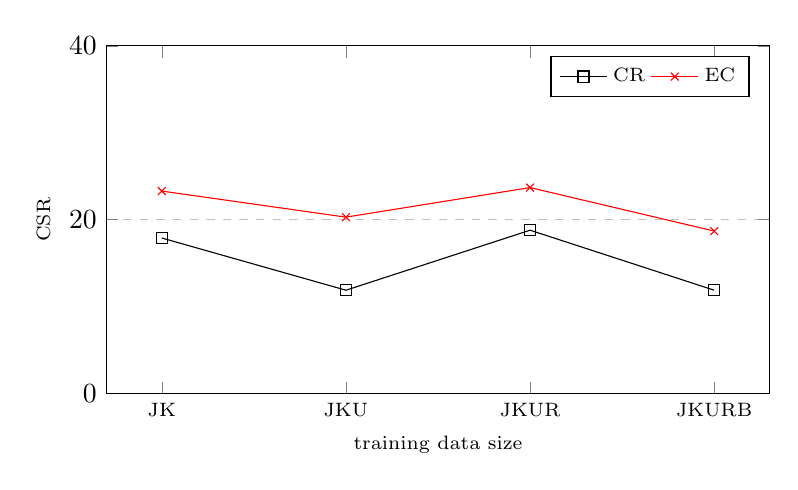
\begin{tikzpicture}
	\begin{axis}[
	title={},
	title style = {font=\scriptsize},
	xlabel={training data size},
	x label style={font=\scriptsize},
	x tick label style={font=\scriptsize},
	xtick=data,
	ylabel={CSR},
	y label style={font=\scriptsize},
	ymin=0, ymax=40,
	symbolic x coords={JK, JKU, JKUR, JKURB},
	ytick={0,20,40},
	legend pos=north east,
	legend style={legend columns=-1, font=\scriptsize},
	ymajorgrids=true,
	grid style=dashed,
	]
	
	\addplot[
	color=black,
	mark=square,
	]
	coordinates {
		(JK,17.9)(JKU,11.9)(JKUR,18.8)(JKURB,11.9)
	};
	
	\addplot[
	color=red,
	mark=x,
	]
	coordinates {
		(JK,23.3)(JKU,20.3)(JKUR,23.7)(JKURB,18.7)
	};
	\legend{CR, EC} 
	\end{axis}
	\end{tikzpicture}
	\caption{$maj/3$ performance v.s. training data size}
	\label{fig:4-datavsmaj3}
\end{figure}

\pgfplotsset{width=10cm,height=6cm,every node near coord/.append style={font=\scriptsize}}
\begin{figure}
	\centering
	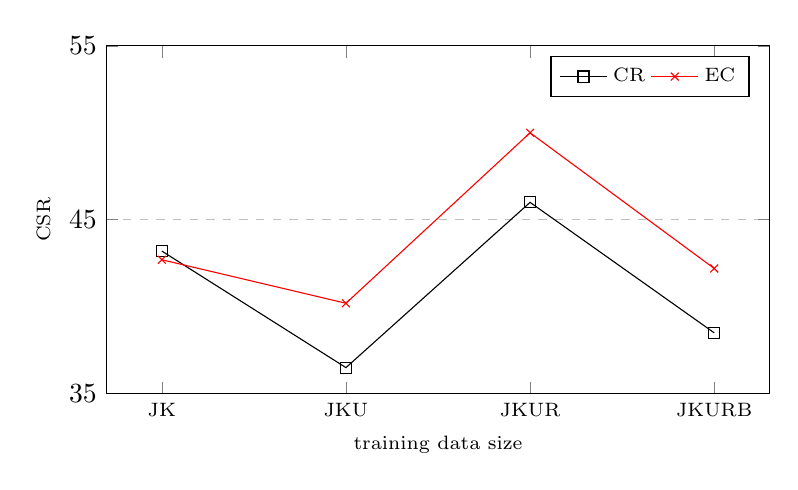
\begin{tikzpicture}
	\begin{axis}[
	title={},
	title style = {font=\scriptsize},
	xlabel={training data size},
	x label style={font=\scriptsize},
	x tick label style={font=\scriptsize},
	xtick=data,
	ylabel={CSR},
	y label style={font=\scriptsize},
	ymin=35, ymax=55,
	symbolic x coords={JK, JKU, JKUR, JKURB},
	ytick={35,45,55},
	legend pos=north east,
	legend style={legend columns=-1, font=\scriptsize},
	ymajorgrids=true,
	grid style=dashed,
	]
	
	\addplot[
	color=black,
	mark=square,
	]
	coordinates {
		(JK,43.2)(JKU,36.5)(JKUR,46.0)(JKURB,38.5)
	};
	
	\addplot[
	color=red,
	mark=x,
	]
	coordinates {
		(JK,42.7)(JKU,40.2)(JKUR,50.0)(JKURB,42.2)
	};
	\legend{CR, EC} 
	\end{axis}
	\end{tikzpicture}
	\caption{$maj/5$ performance v.s. training data size. Input: chromagram}
	\label{fig:4-datavsmaj5}
\end{figure}

A reasonable conjecture of why this might happen in EC is that the ground-truth labeling of chords, specifically in datasets U and B, are not consistent. Particularly, some inversion chords may be mislabeled as root positions or vice versa (for example, $maj/3$ labeled as $maj$ or vice versa) as they are sometimes easily confusable. There is a very good chance that this might happen and thus it introduces noise in the data, which could eventually blur the trained model's classification boundaries between these confusing chord pairs.
%While this conjecture might be true, a more solid justification demands a much deeper investigation into the labels of these datasets and the chord confusion matrices between these confusing pairs mentioned above. (say it when you have the data)


\subsection{System comparison}

\begin{table}[htb]
	\caption{Comparison between the proposed systems and Chordino - overall performance. Input: chromagram}
	\label{tab:4-cpcd}
	\centering
	\scriptsize
	\begin{tabular}{|c|c|c|c|c|c|c|c|c|c|c|c|c|c|}\hline
		System & \textit{MajMin} & \textit{MajMinBass} & \textit{Sevenths} & \textbf{\textit{SeventhsBass}} & Segmentation Quality\\ \hline
		JKURB & 70.6 & 68.7 & 56.3 & 54.7 & 78.0\\ \hline
		JKURB* & 70.1 & 68.2 & \textbf{57.6} & \textbf{56.0} & 76.8\\ \hline
		Chordino & \textbf{72.4} & \textbf{69.1} & 55.8 & 52.8 & \textbf{83.8}\\ \hline
	\end{tabular}
\end{table}

Finally, we would like to know how good is this LVACE approach compared with existing ones. Chordino\cite{cannam2013mirex} is used as a comparison baseline. It has a similar feature extraction module as the proposed systems and it supports a similar set of large vocabulary, which most of other ACE systems do not support. Chordino is an expert system (non-machine learning) that represents a very high standard \cite{deng2016chord} in terms of large vocabulary balanced performance.

Table~\ref{tab:4-cpcd} shows the comparison, in which there are two systems trained with the largest possible amount of data with different training schemes. In terms of overall performances, the proposed systems slightly outperform Chordino in terms of the strictest \textit{SeventhsBass} score, but slightly underperform Chordino in the more relaxed \textit{MajMin} and \textit{MajMinBass} scores.

% may need to change some wordings here, to sloppy
A large margin is found in segmentation quality, in which Chordino scores 5.3 and 7 points higher than the proposed systems. As noted previously, the segmentation quality is indeed a problem in this end-to-end approach. One could expect a boost of overall performance as well as balanced performance if the segmentation quality score could be raised to at least Chordino's level.

\begin{table}[htb]
	\caption{Comparison between the proposed systems and Chordino - long-tail and balanced performance. Input: chromagram}
	\label{tab:4-cpcd-2}
	\centering
	\scriptsize
	\begin{tabular}{|c|c|c|c|c|c|c|c|c|c|c|c|c|c|}\hline
		System & \textit{maj/5} & \textit{maj/3} & \textit{7/b7} & \textit{ACQA} \\ \hline
		JKURB & 11.9 & 38.5 & 4.9 & 14.7\\ \hline
		JKURB* & 18.7 & \textbf{42.2} & 24.0 & \textbf{18.4}\\ \hline
		Chordino & \textbf{ 27.6} & 29.8 & \textbf{24.4} & \textbf{20.9}\\ \hline
	\end{tabular}
\end{table}
Table~\ref{tab:4-cpcd-2} shows another set of comparisons in terms of long-tail and balanced performance. The CR system underperforms Chordino in all the presented categories except for $maj/3$.	The EC system outperforms Chordino in $maj/3$ and gets very close to Chordino in both $7/b7$ and $ACQA$. The latter results are very promising as they showcase that an end-to-end large vocabulary chord sequence classifier (JKURB*) could achieve a long-tail and balanced performance close to a manually engineered expert system (Chordino), with the help of the proposed even chance training scheme.

\section{Summary}\label{sec:4-concln}
This chapter proposes an end-to-end ``local feature extraction - global classification'' BLSTM-RNN based ACE system that supports SeventhsBass vocabulary. This system has a handcrafted feature extraction process, and can be compared with Chordino in a statistically fair way. To cater for large vocabulary recognition, an even chance training scheme is designed. Several variants of the system are trained and implemented. Evaluation results show some variants largely outperform Chordino in terms of large vocabulary scores, and they are almost as good as Chordino in terms of small vocabulary scores, despite having much worse segmentation qualities. It can be concluded that the proposed BLSTM-RNN architecture is better than the dedicated handcrafted GMM-HMM in terms of large vocabulary sequence modeling, but it suffers from bad sequence segmentation.

Through detail analysis of the results, a plausible issue of annotation inconsistency is identified. As suggested in Chapter~\ref{cp:background}, a workaround would be to always use annotations provided by one single source/annotator, or, to the other extreme, always use multiple annotators and apply majority vote or data fusion. But eventually, the ultimate evaluation tool may remain a fully subjective one, that let user experience to judge system performance.

Even chance training has been demonstrated very efficient in improving long-tail symbol recalls. It also boosts some VERY long-tail cases from zero score to non-zero. However, it sacrifices the performances of large population chords, and thus downgrades the overall performances in all but the versatility category.

To improve this system, the key thing to be done is to improve RNN's segmentation quality, since it determines an upper-bound of all other system performance, and the scores of all other metrics scale in proportion to segmentation quality. This can possibly be done through a dedicated segmentation training pass, a deeper RNN model, or combination of a segmentation-RNN with a annotation-RNN in a hierarchical way.




% ---------------------------------------------------------------------------
%: ----------------------- end of thesis sub-document ------------------------
% ---------------------------------------------------------------------------

